% This template is translated by Trang Nguyen Minh and Hanh Nguyen Hong, from BKIC 611 lab with love <3
%%%%%%%%%%%%%%%%%%%%%%%%%%%%%%%%%%%%%%%%%%%%%%%%%%%%%%%
\documentclass{article} % 
\usepackage[utf8]{inputenc}
\usepackage[T5]{fontenc} % Vietnamese
\usepackage[fontsize=13pt]{scrextend} % Set fontsize=13pt
%\usepackage[paperheight=29.7cm,paperwidth=21cm,right=2cm,left=3cm,top=2cm,bottom=2.5cm]{geometry}% Chuẩn A4, căn lề phải, trái, trên, dưới.
\usepackage[paperheight=29.7cm,paperwidth=21cm,right=2cm,left=3cm,top=2cm,bottom=2.5cm,twoside]{geometry}% Chuẩn A4, căn lề phải, trái, trên, dưới.
\usepackage{mathptmx} % Time New Roman
\usepackage{graphicx} 
\usepackage{float} 
\usepackage{tikz}
\usetikzlibrary{calc} 
\usepackage{indentfirst} 
\renewcommand{\baselinestretch}{1.2} % Line space 1.2
\setlength{\parskip}{6pt} % Spacing after
\setlength{\parindent}{1cm} % Set khoảng cách thụt đầu dòng mỗi đoạn
\usepackage{titlesec} 
\setcounter{secnumdepth}{4} % 4 Heading
\titlespacing*{\section}{0pt}{0pt}{30pt} % Heading 1
\titleformat*{\section}{\fontsize{16pt}{19.2pt}\selectfont \bfseries \centering}

\titlespacing*{\subsection}{0pt}{10pt}{0pt} % Heading 2
\titleformat*{\subsection}{\fontsize{14pt}{16.8pt}\selectfont \bfseries}

\titlespacing*{\subsubsection}{0pt}{10pt}{0pt} % Heading 3
\titleformat*{\subsubsection}{\fontsize{13pt}{15.6pt}\selectfont \bfseries \itshape}

\titlespacing*{\paragraph}{0pt}{10pt}{0pt} % Heading 4
\titleformat*{\paragraph}{\fontsize{13pt}{15.6pt}\selectfont \itshape}

\renewcommand{\figurename}{\fontsize{12pt}{0pt}\selectfont \bfseries Figure}
\renewcommand{\thefigure}{\thesection.\arabic{figure}}
\usepackage[font=bf]{caption}
\captionsetup[figure]{labelsep=space}

\renewcommand{\tablename}{\fontsize{12pt}{0pt}\selectfont \bfseries Table}
\renewcommand{\thetable}{\thesection.\arabic{table}}
\captionsetup[table]{labelsep=space}

\usepackage{multicol,multirow,tabularx}
\newcolumntype{s}{>{\hsize=.3\hsize}X}
\newcolumntype{y}{>{\hsize=.4\hsize}X}
\newcolumntype{d}{>{\hsize=.1\hsize}X}
\newcolumntype{a}{>{\hsize=1.1\hsize}X}
\newcolumntype{g}{>{\hsize=5\hsize}X}
\newcolumntype{C}[1]{>{\hsize=#1\hsize\centering\arraybackslash}X}
\newcolumntype{R}[1]{>{\hsize=#1\hsize\raggedleft\arraybackslash}X}
\newcolumntype{L}[1]{>{\hsize=#1\hsize\raggedright\arraybackslash}X}
\renewcommand{\tabularxcolumn}[1]{>{\small}m{#1}}

\renewcommand{\theequation}{\thesection.\arabic{equation}}
\newtheorem{theorem}{Theorem}[section]
\newtheorem{defn}[theorem]{Defenition}
\newtheorem{corollary}[theorem]{Corollary}
\newtheorem{lemma}[theorem]{Lemma}

\usepackage{lipsum} % Thư viện tạo chữ linh tinh.
\renewcommand{\contentsname}{TABLE OF CONTENTS}
\renewcommand{\listfigurename}{LIST OF FIGURES}
\renewcommand{\listtablename}{LIST OF TABLES}
\renewcommand{\refname}{REFERENCES}

\usepackage[unicode]{hyperref}
\usepackage{colortbl}
\definecolor{LightCyan}{rgb}{0.88,1,1}
\usepackage{forloop}
\newcounter{loopcntr}
\newcommand{\rpt}[2][1]{\forloop{loopcntr}{0}{\value{loopcntr}<#1}{#2}}

\usepackage[ddmmyyyy]{datetime}
\usepackage{amsmath}
\usepackage{nameref}
\usepackage{rotating}
\usepackage{bm}
\DeclareRobustCommand{\vect}[1]{\bm{#1}}
\pdfstringdefDisableCommands{%
  \renewcommand{\vect}[1]{#1}%
}

\begin{document}

\thispagestyle{empty}
\begin{tikzpicture}[overlay,remember picture]
\draw [line width=3pt]
    ($ (current page.north west) + (3.0cm,-2.0cm) $)
    rectangle
    ($ (current page.south east) + (-2.0cm,2.5cm) $);
\draw [line width=0.5pt]
    ($ (current page.north west) + (3.1cm,-2.1cm) $)
    rectangle
    ($ (current page.south east) + (-2.1cm,2.6cm) $); 
\end{tikzpicture}
\begin{center}
\vspace{-12pt} HANOI UNIVERSITY OF SCIENCE AND TECHNOLOGY \\
\textbf{\fontsize{14pt}{0pt}\selectfont SCHOOL OF ELECTRICAL AND ELECTRONIC ENGINEERING}
\vspace{1cm}
 \begin{figure}[H]
     \centering
     
\includegraphics[width=0.15\textwidth]{Figures/logoBK.png}
 \end{figure}
\vspace{1cm}
\textbf{\fontsize{25pt}{0pt}\selectfont GRADUATION THESIS}
\vspace{1cm}
\end{center}
\begin{center}
    \textbf{\fontsize{21pt}{0pt}\selectfont Simulation of the OFDM system using channel coding, LMSE and 64 QAM modulation. }
\vspace{7pt}
\begin{table}[H]
    \centering
    \begin{tabular}{l l l}
        Full Names & Class & Student ID \\
        Ngô Văn Cảnh & CTTT Dien Tu 01 K64 & 20193204 \\
        Nguyễn Ngọc Dũng & CTTT Dien Tu 01 K64 & 2019xxxx \\
        Bạch Vũ Thái Dương & CTTT Dien Tu 01 K64 & 2020xxxx \\
        Hoàng Thế Nguyên & CTTT Dien Tu 01 K64 & 2018xxxx \\
    \end{tabular}
\end{table}
\vspace{1.5cm}
\begin{table}[H]
    \centering
    \begin{tabular}{l l}
        \fontsize{14pt}{0pt}\selectfont Supervisor: & \fontsize{14pt}{0pt}\selectfont Dr. Nguyen Van Duc \\
        {} & Dr. Nguyen Thu Nga \hspace{5pt} \\
    \end{tabular}
\end{table}
\vspace{1.5cm}
\fontsize{14pt}{0pt}\selectfont Hanoi, 26/12/2023
\end{center}

 

%\section*{PLEDGE}
\thispagestyle{empty}
abc ..

\vspace{6pt}
\hspace{7cm}Hanoi, 00/00/2023

\hspace{9cm}\textbf{Student}

\vspace{2cm}
\hspace{8.3cm}\textbf{NGUYỄN vĂN A}
\cleardoublepage 

\addtocontents{toc}{\protect\thispagestyle{empty}}
\tableofcontents 
\thispagestyle{empty}
\cleardoublepage

\pagenumbering{roman} % Đánh số thứ tự la mã
\section*{LIST OF ABBREVIATIONS}
\phantomsection \addcontentsline{toc}{section}{\numberline {} LIST OF ABBREVIATIONS}

\begin{tabularx}{\textwidth}{ L{0.4} L{1.3} L{1.3} }
    OFDM    & Orthogonal Frequency Division Multiplexing \\
    QAM     & Quadrature Amplitude Modulation \\
    LMSE    & Least Mean Square Equalizer \\ % Linear Minimum Mean Square Error
    FFT     & Fast Fourier Transform \\
    IFFT    & Inverse Fast Fourier Transform \\
    BER     & Bit Error Rate \\
    SER     & Symbol Error Rate \\
    PSK     & Phase Shift Keying \\
    FDM     & Frequency Division Multiplexing \\
    CP      & Cyclic Prefix \\
    SNR     & Signal to Noise Ratio \\
    LPF     & Low Pass Filter \\

\end{tabularx}

\newpage 

{\let\oldnumberline\numberline
\renewcommand{\numberline}{Figure~\oldnumberline}
\listoffigures} 
\phantomsection\addcontentsline{toc}{section}{\numberline {} LIST OF FIGURES}
\newpage

 %Tạo danh mục bảng biểu.
{\let\oldnumberline\numberline
\renewcommand{\numberline}{Table~\oldnumberline}
\listoftables}
\phantomsection\addcontentsline{toc}{section}{\numberline {} LIST OF TABLES}
\newpage

% \section*{ABSTRACT}
% This project focuses on the comprehensive simulation and performance analysis of an Orthogonal Frequency Division Multiplexing (OFDM) communication system enhanced with channel coding, Linear Minimum Mean Square Error (LMSE) equalization, and 64 Quadrature Amplitude Modulation (64 QAM). OFDM, a widely used modulation technique, divides the frequency spectrum into orthogonal subcarriers, making it resilient to channel impairments.

% The project's primary objectives include the implementation of channel coding techniques, such as Reed-Solomon or convolutional coding, to introduce redundancy for error correction. Additionally, LMSE equalization is employed to mitigate the impact of channel distortions, enhancing the overall system robustness.

% The modulation aspect of the project involves the utilization of 64 QAM, a higher-order modulation scheme, allowing for increased data rates. The combination of these techniques aims to optimize the system's spectral efficiency and error resilience in the presence of noise, interference, and fading channels.

% The simulation workflow encompasses the generation of random binary data, channel coding, 64 QAM modulation, OFDM modulation, channel modeling, additive white Gaussian noise (AWGN) introduction, LMSE equalization, and subsequent demodulation. The Bit Error Rate (BER) or Symbol Error Rate (SER) is then estimated to quantify the system's performance.

% The results of this simulation will provide valuable insights into the effectiveness of the integrated components in enhancing the reliability and efficiency of the OFDM communication system. The project's findings have implications for the design and optimization of communication systems in various wireless and broadband applications.

Modern communication systems face challenges of inter-symbol interference (ISI) and inter-carrier interference (ICI), particularly in single carrier systems with long symbol periods or multicarrier systems with closely spaced carriers. Orthogonal Frequency Division Multiplexing (OFDM) emerges as a solution by combining numerous low data rate carriers to construct a high data rate communication system. The orthogonality of carriers in OFDM enables close spacing without ICI, addressing the limitations of traditional multicarrier systems.

This project aims to demonstrate and explore the feasibility of an OFDM system, investigating the impact of key parameters on its performance. A Python program is developed for simulating a basic OFDM system, providing insights into its mechanisms and characteristics.
% The report is structured to offer a theoretical background in Chapter 1, essential for understanding the project's concepts. Chapter 2 details the design and implementation of the OFDM system, while Chapter 3 presents the simulation results and performance evaluation.

The comprehensive study of OFDM presented in this project contributes to the understanding of its advantages and limitations, laying the foundation for further research and applications in the evolving landscape of wireless communication.
\newpage
\cleardoublepage

\section*{WORK CONTRIBUTION}
\phantomsection \addcontentsline{toc}{section}{\numberline {} WORK CONTRIBUTION}

\begin{table}[!ht]
\begin{tabular}{|l|l|l|}
    \hline
    \textbf{No.}    & \textbf{Job}      & \textbf{Name} \\ \hline
    1               & Report            & Ngo Van Canh  \\ \hline
    2               & Slide             & Nguyen Ngoc Dung \& Ngo Van Canh \\ \hline
\end{tabular}
\end{table}

\newpage 

\pagenumbering{arabic} % Đánh số thứ tự 1,2,3...

\section*{CHAPTER 1. INTRODUCTION}
\addcontentsline{toc}{section}{\numberline{}CHAPTER 1. INTRODUCTION}
\setcounter{section}{1}
\setcounter{subsection}{0}
\setcounter{figure}{0}
\setcounter{table}{0}

In a single carrier communication system, the symbol period must be much 
greater than the delay time in order to avoid inter-symbol interference (ISI) \cite{b1}. Since 
data rate is inversely proportional to symbol period, having long symbol periods 
means low data rate and communication inefficiency. A multicarrier system, such as 
FDM (aka: Frequency Division Multiplexing), divides the total available bandwidth 
in the spectrum into sub-bands for multiple carriers to transmit in parallel \cite{b2}. An 
overall high data rate can be achieved by placing carriers closely in the spectrum. 
However, inter-carrier interference (ICI) will occur due to lack of spacing to separate 
the carriers. To avoid inter-carrier interference, guard bands will need to be placed in 
between any adjacent carriers, which results in lowered data rate. 

OFDM (aka: Orthogonal Frequency Division Multiplexing) is a multicarrier 
digital communication scheme to solve both issues. It combines a large number of 
low data rate carriers to construct a composite high data rate communication system. 
Orthogonality gives the carriers a valid reason to be closely spaced, even overlapped, 
without inter-carrier interference. Low data rate of each carrier implies long symbol 
periods, which greatly diminishes inter-symbol interference \cite{b3}. 

Although the idea of OFDM started back in 1966 \cite{b4}, it has never been widely 
utilized until the last decade when it “becomes the modem of choice in wireless 
applications” \cite{b5}. It is now interested enough to experiment some insides of OFDM. 

The objective of this project is to demonstrate the concept and feasibility of an 
OFDM system, and investigate how its performance is changed by varying some of 
its major parameters. This objective is met by developing a MATLAB program to 
simulate a basic OFDM system. From the process of this development, the 
mechanism of an OFDM system can be studied; and with a completed MATLAB 
program, the characteristics of an OFDM system can be explored. 
\newpage
\section*{CHAPTER 2: BACKGROUND}
\addcontentsline{toc}{section}{\numberline{}CHAPTER 2: BACKGROUND}
\setcounter{section}{2}
\setcounter{subsection}{0}
\setcounter{figure}{0}
\setcounter{table}{0}

\subsection{OFDM Basics}

In digital communications, information is expressed in the form of bits. The term symbol refers to a collection, in various sizes, of bits. OFDM data are generated by taking symbols in the spectral space using M-PSK, QAM, etc, and convert the spectra to time domain by taking the Inverse Discrete Fourier Transform (IDFT). Since Inverse Fast Fourier Transform (IFFT) is more cost effective to implement, it is usually used instead \cite{b3}. Once the OFDM data are modulated to time signal, all carriers transmit in parallel to fully occupy the available frequency bandwidth. During modulation, OFDM symbols are typically divided into frames, so that the data will be modulated frame by frame in order for the received signal be in sync with the receiver. Long symbol periods diminish the probability of having inter-symbol interference, but could not eliminate it. To make ISI nearly eliminated, a cyclic extension (or cyclic prefix) is added to each symbol period. An exact copy of a fraction of the cycle, typically 25\% of the cycle, taken from the end is added to the front. This allows the demodulator to capture the symbol period with an uncertainty of up to the length of a cyclic extension and still obtain the correct information for the entire symbol period.

\begin{figure}[ht]
    \centering
    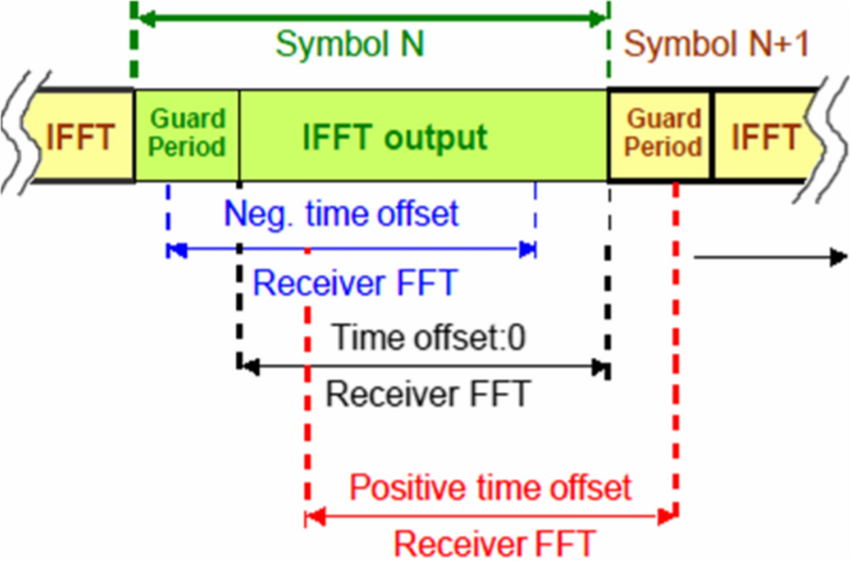
\includegraphics[width=0.5\textwidth]{Figures/Cyclic-extension-tolerance.png}
    \caption{\bfseries\centering\fontsize{13pt}{0pt}\selectfont Cyclic-extension-tolerance}
    \label{Cyclic-extension-tolerance}
\end{figure}

As shown in Figure \ref{Cyclic-extension-tolerance}, a guard period, another name for the cyclic extension, is the amount of uncertainty allowed for the receiver to capture the starting point of a symbol period, such that the result of FFT still has the correct information. In Figure 2, a comparison between a precisely detected symbol period and a delayed detection illustrates the effectiveness of the cyclic extension.

\begin{figure}[ht]
    \centering
    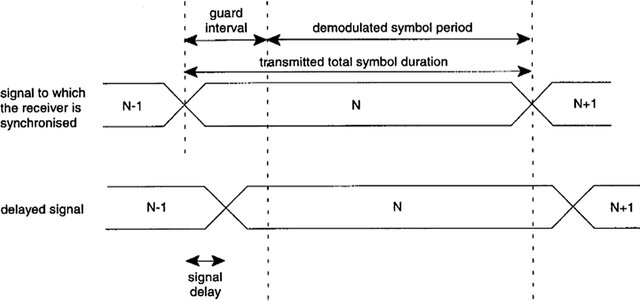
\includegraphics[width=\textwidth]{Figures/Effectiveness-of-cyclic-extension.jpg}
    \caption{\bfseries\centering\fontsize{13pt}{0pt}\selectfont Effectiveness-of-cyclic-extension}
    \label{Effectiveness-of-cyclic-extension}
\end{figure}

\subsection{OFDM Parameters and Characteristics}

\subsubsection{Complexity}

The number of carriers in an OFDM system is not only limited by the available spectral bandwidth, but also by the IFFT size, which is determined by the complexity of the system. The more complex (also more costly) the OFDM system is, the higher IFFT size it has; thus a higher number of carriers can be used, and higher data transmission rate achieved. The choice of M-PSK modulation varies the data rate and Bit Error Rate (BER). The higher order of PSK leads to larger symbol size, thus less number of symbols needed to be transmitted, and higher data rate is achieved. But this results in a higher BER since the range of 0-360 degrees of phases will be divided into more sub-regions, and the smaller size of sub-regions is required, thereby received phases have higher chances to be decoded incorrectly. OFDM signals have high peak-to-average ratio, therefore it has a relatively high tolerance of peak power clipping due to transmission limitations.

\subsubsection{Orthogonality}

The key to OFDM is maintaining orthogonality of the carriers. If the integral of the product of two signals is zero over a time period, then these two signals are said to be orthogonal to each other. Two sinusoids with frequencies that are integer multiples of a common frequency can satisfy this criterion. Therefore, orthogonality is defined by :

\begin{equation}\label{eq1}
    \int_{0}^{T} cos(2 \pi n f_o t) cos(2 \pi m f_o t) \,dt = 0 \quad (n \neq m) 
\end{equation}

Where $n$ and $m$ are two unequal integers; $f_o$ is the fundamental frequency; $T$ is the period over which the integration is taken. For OFDM, $T$ is one symbol period and $f_o$ set to to $\frac{1}{T}$ for optimal effectiveness.

\subsubsection{Advantages and Disadvantages}

Upgrading and optimizing algorithms, OFDM systems provide highly advantageous features for wireless transmission and transceiver system design:

\begin{itemize}
    \item  Complete Elimination of ISI (InterSymbol Interference): OFDM systems can entirely eliminate ISI by employing an appropriate Guard Interval, thus mitigating multipath distortion.
    \item Suitable for High-Speed Transmission Systems: OFDM is well-suited for high-speed transmission systems due to the significant reduction in Frequency Selectivity compared to single-carrier transmission. This reduction minimizes the impact of frequency-selective fading.
    \item Simple Receiver Structure: OFDM systems boast a simple receiver structure, contributing to ease of implementation.
\end{itemize}
However, OFDM technology also has its drawbacks that need careful consideration and practical research for designing a system suitable for specific purposes:
\begin{itemize}
    \item Uneven Amplitude Envelope: The amplitude envelope of the signal is uneven, causing nonlinear distortion in power amplifiers at the transmitter and receiver.
    \item Guard Interval Impact on Transmission Efficiency: While the guard interval is used to eliminate ISI, it also reduces transmission efficiency due to wasting power on transmitting useless signals.
    \item Orthogonality Conditions between Subcarriers: The requirement for orthogonality between subcarriers makes the system susceptible to the effects of Doppler, frequency offset, and time offset due to synchronization errors.
\end{itemize}
These challenges require careful consideration and research to optimize the performance of the OFDM system under real-world conditions and ensure that the drawbacks do not significantly affect transmission quality

\newpage
\section*{CHAPTER 3:  DESIGN AND IMPLEMENTATION}
\addcontentsline{toc}{section}{\numberline{}CHAPTER 3: DESIGN AND IMPLEMENTATION}
\setcounter{section}{3}
\setcounter{subsection}{0}
\setcounter{figure}{0}
\setcounter{table}{0}

\subsection{OFDM Modulation method and transceiver architechure}
Orthogonal Frequency Division Multiplexing (OFDM) modulation is based on the Frequency Division Multiplexing (FDM) technique, with the key distinction that the subcarrier waves are placed orthogonally to each other. With this orthogonality, their signal spectra overlap without affecting the demodulation process at the receiver. The signal spectrum of a system of subcarrier waves is illustrated in Figure \ref{Spectrum} \cite{b6}.

\begin{figure}[htbp]
    \centering
    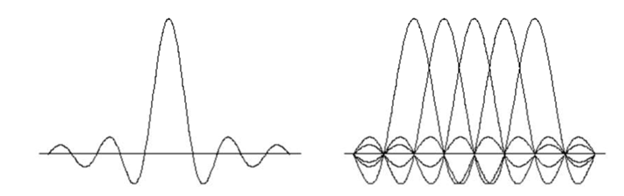
\includegraphics[width=\textwidth]{Figures/Spectrum.png}
    \caption{\bfseries\centering\fontsize{13pt}{0pt}\selectfont Spectrum of a single subcarrier (left) and 5 subcarriers (right)}
    \label{Spectrum}    
\end{figure}

As shown in Figure \ref{Spectrum}, the signal spectrum of each subcarrier channel has the form of $\frac{sin(x)}{x}$. The subcarriers are distributed evenly across the frequency range, ensuring that the peak points of one channel coincide with the null points of adjacent subcarrier channels. In the OFDM system, the signals, after passing through the digital modulator, undergo an Inverse Fast Fourier Transform (IFFT) to form OFDM symbols. The use of IFFT allows the OFDM modulator to simultaneously modulate multiple channels, a task that is challenging with FDM modulators.

\begin{figure}[htbp]
    \centering
    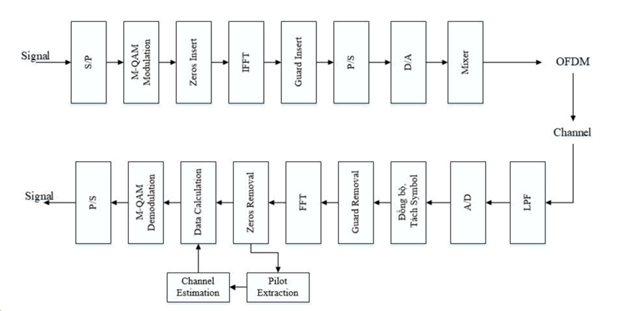
\includegraphics[width=\textwidth]{Figures/Block-diagram.png}
    \caption{\bfseries\centering\fontsize{13pt}{0pt}\selectfont Block diagram of the OFDM system}
    \label{Block diagram}    
\end{figure}

Principles of operation for each block:
\begin{itemize}
    \item S/P (Serial to Parallel): Converts serial data into parallel data, splitting high-speed bit streams into K lower-speed bit streams, where K is the number of subcarrier waves in the system.
    \item M-QAM Modulation: Utilizes QAM modulation to map pairs of bits into complex signals in the QAM signal constellation. The modulation level M is chosen based on different transmission systems.
    \item Zero Insertion: Inserts virtual subcarriers to ensure the DC component's average value is zero and creates a frequency guard band between information systems to avoid Intercarrier Interference (ICI).
    \item IFFT (Inverse Fast Fourier Transform): Performs a fast implementation of the Inverse Discrete Fourier Transform, transforming signals from the time domain to the frequency domain, creating orthogonal subcarrier waves.
    \begin{equation}
        x_n = \frac{1}{N} \sum_{k=0}^{N-1} X_k . e^\frac{j2\pi kn}{N}
    \end{equation}
    \item Guard Insertion: Inserts a guard interval to counteract Inter-Symbol Interference (ISI). ISI arises from the influence of multipath effects when symbols arriving later interfere with symbols arriving earlier. The guard interval length depends on the transmission channel and follows the principle of copying a portion of the signal sequence that needs to be transmitted and appending it to the beginning of the signal.
    \item P/S (Parallel to Serial): Converts parallel data back to serial, returning the signal stream to its original continuous form for transmission.
    \item Mixer: Combines the signal with carrier waves before sending it to the antenna. OFDM modulation uses two different Mixers for two streams of real and complex signals from the P/S block. These two signal streams are multiplied successively with carrier waves and then added at the Mixer's output.
    \item LPF (Low Pass Filter): Low-pass filter that brings the signal back to baseband.
    \item D/A, A/D: Converts signals from digital to analog and analog to digital for long-distance transmission. The signal after D/A conversion is an analog baseband signal with a bandwidth depending on the sampling frequency in the D/A converter. At the receiver, an A/D converter is used to obtain digital signals for decoding.
    \item Pilot Extraction, Channel Estimation: Based on pilot signals, the receiver estimates the transmission channel using estimation algorithms.
    \item 64-QAM Modulation/Demodulation: Maps binary sequences to complex signals characteristic of points in the QAM signal constellation. As illustrated in Figure \ref{Constellation}, each bit sequence corresponds to one point on the complex plane. Quadrature Amplitude Modulation (QAM) is a modulation technique that combines amplitude modulation and phase modulation. Compared to other modulation types, QAM signals can resist noise effectively because the receiver can differentiate based on both amplitude and phase. The symbol constellation of QAM signals has larger amplitude and phase differences than other modulation types with the same number of levels M, making it less susceptible to interference when symbols overlap.
\end{itemize}

\begin{figure}[htbp]
    \centering
    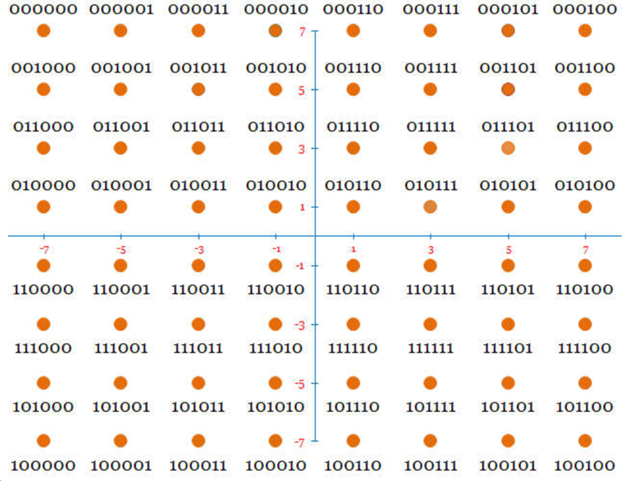
\includegraphics[width=\textwidth]{Figures/64-QAM-Constellation.png}
    \caption{\bfseries\centering\fontsize{13pt}{0pt}\selectfont 64-QAM Constellation}
    \label{Constellation}   
\end{figure}
\newpage
\section*{CHAPTER 4: SIMULATION AND RESULTS}
\addcontentsline{toc}{section}{\numberline{}CHAPTER 4: SIMULATION AND RESULTS}
\setcounter{section}{4}
\setcounter{subsection}{0}
\setcounter{figure}{0}
\setcounter{table}{0}

In this project, we're using a python script to simulate the 64 QAM OFDM system. A 3 channels bitmap image is used as source input. Another bitmap iamge file will be generated at the end of the simulation as the output.

\subsection{Configurations and Parameters set up}

\begin{enumerate}
    \item $K = 64$ : The number of subcarriers, describes how many subcarriers are available in the OFDM system.
    \item $CP = K//$4 : The length of the cyclic prefix (CP) denotes the number of samples that are copied from the end of the modulated block to the beginning, to yield a cyclic extension of the block.
    \item $P = 8$ : The number of pilots in the OFDM symbol, describes how many carriers are used to transmit known information (i.e. pilots). Pilots will be used at the receiver to estimate the wireless channel between transmitter and receiver.
    \item $pilotValue = 3+3j$ : The known value each pilot transmits
\end{enumerate}

After that, we need to define some index sets that describe which carriers transmit pilots and which carriers contain payload.

\begin{figure}[htbp]
    \centering
     \begin{subfigure}[t]{.49\linewidth}
        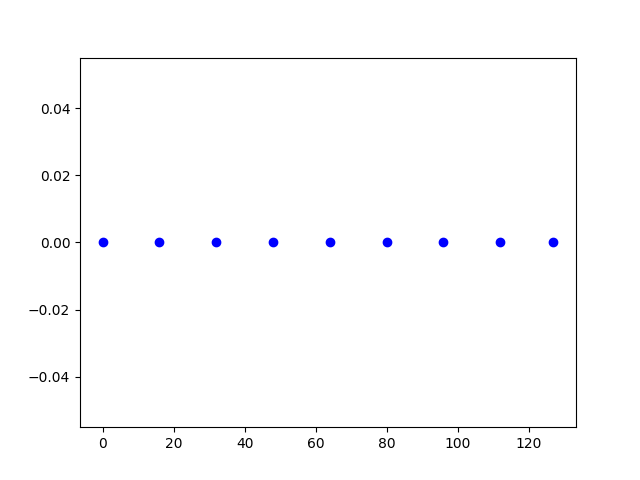
\includegraphics[width=\linewidth]{../Source/results/pilotCarriers.png}
        \caption{Pilot Carriers}
        \label{pilotCarriers}
    \end{subfigure}
    % \hfil
    \begin{subfigure}[t]{0.49\linewidth}
        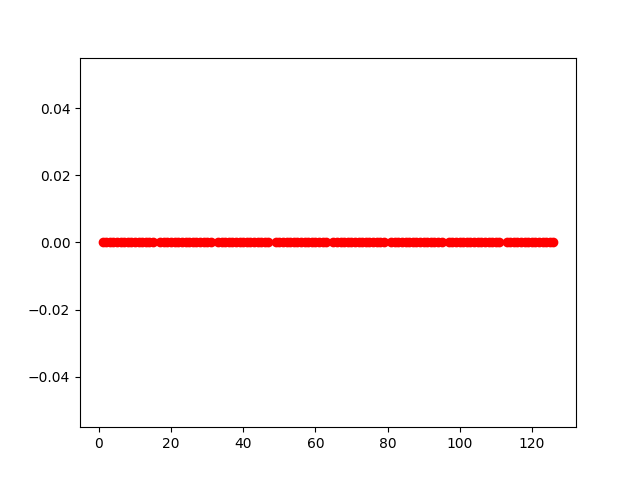
\includegraphics[width=\linewidth]{../Source/results/dataCarriers.png}
        \caption{Data Carriers}
        \label{dataCarriers}
    \end{subfigure}
    \caption{The Carriers transmit pilots and which carriers contain payload}
\end{figure}

Let's define the modulation index $\mu$ and the corresponding mapping table. We consider 64QAM transmission, i.e. we have $\mu=6$ bits per symbol. Furthermore, the mapping from groups of 6 bits to a 64QAM constellation symbol shall be defined in mapping table.

\begin{figure}[ht]
    \centering
    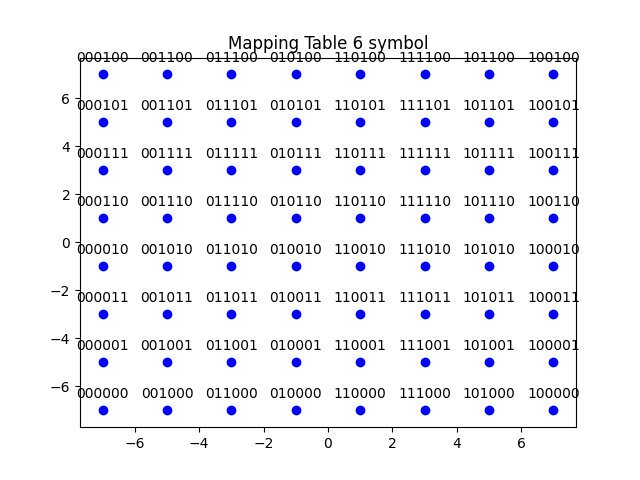
\includegraphics[width=\textwidth]{../Source/results/mapping.png}
    \caption{64-QAM Constellation with gray-mapping}
    \label{mapping}
\end{figure}

In Figure \ref{mapping}, we have plotted the 64-QAM constellation, along with the bit-labels.
Int Gray-mapping, two adjacent constellation symbols differ only by one bit and the other 5 bits remain the same. This technique helps to minimize bit-errors, in case a wrong constellation symbol is detected: Most probably, symbol errors are "off-by-one" errors, i.e. a symbol next to the correct symbol is detected. Then, only a single bit-error occurs.

\subsection{OFDM Transmitter}

Now, that we have defined the necessary parameters for our OFDM example, let us consider the blocks in the OFDM system. As mention earlier, the input b is a 3 channels, 256x256 bitmap image (Figure \ref{input}). To fully transmitt this imgae, we need 256*256*3=196608 bits.

\begin{figure}[htbp]
    \centering
    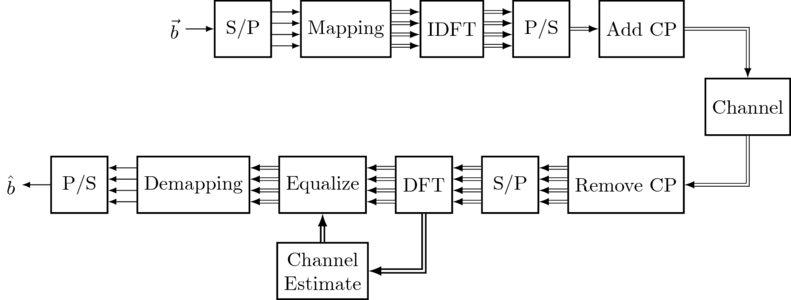
\includegraphics[width=\textwidth]{Figures/Block-diagram-2.png}
    \caption{Block diagram of the OFDM system}
    \label{Block diagram 2}
\end{figure}

\begin{figure}[htbp]
    \centering
    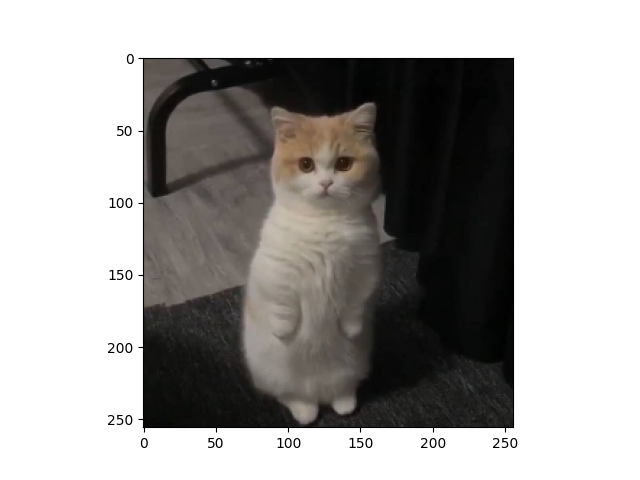
\includegraphics[width=\textwidth]{../Source/results/input.png}
    \caption{Input image}
    \label{input}
\end{figure}

These bits are now sent to a serial-to-parallel converter, which groups the bits for the OFDM frame into a groups of $\mu$ bits (i.e. one group for each subcarrier). The bits groups are then sent to the mapper. The mapper converts the groups into complex-valued constellation symbols according to the mapping\_table (Figure \ref{mapping}).

The next step is the allocation of different subcarriers with data and pilots. For each subcarrier we have defined wether it carries data or a pilot by the arrays dataCarriers and pilotCarriers. Now, to create the overall OFDM data, we need to put the data and pilots into the OFDM carriers. Now, the OFDM carriers contained in OFDM\_data can be transformed to the time-domain by means of the IDFT operation.

Subsequently, we add a cyclic prefix to the symbol. This operation concatenates a copy of the last CP samples of the OFDM time domain signal to the beginning. This way, a cyclic extension is achieved. The CP fulfills two tasks:
\begin{enumerate}
    \item It isolates different OFDM blocks from each other when the wireless channel contains multiple paths, i.e. is frequency-selective.
    \item It turns the linear convolution with the channel into a circular one. Only with a circular convolution, we can use the single-tap equalization OFDM is so famous for.
\end{enumerate}

After this step :
\begin{itemize}
    \item Number of OFDM carriers in frequency domain: 128
    \item Number of OFDM samples in time-domain before CP: 128
    \item Number of OFDM samples in time domain with CP: 160
\end{itemize}

Now, the signal is sent to the antenna and sent over the air to the receiver. In between both antennas, there is the wireless channel. We model this channel as a static multipath channel with impulse response channelResponse. Hence, the signal at the receive antenna is the convolution of the transmit signal with the channel response. Additionally, we add some noise to the signal according to the given SNR value. Figure \ref{tx_rx} shows the TX and RX signal with SNR value = 20db.

\begin{figure}[htbp]
    \centering
    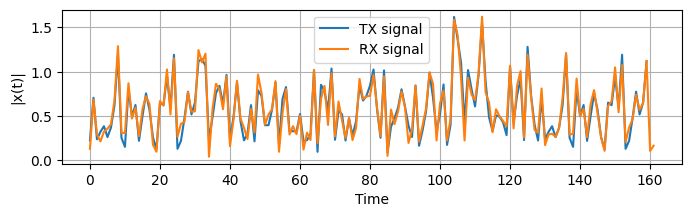
\includegraphics[width=\textwidth]{../Source/results/tx_rx.png}
    \caption{TX and RX signal with SNR value = 20db}
    \label{tx_rx}
\end{figure}

\subsection{OFDM Receiver}

Now, at the receiver the CP is removed from the signal and a window of $K$ samples is extracted from the received signal. Afterwards, the signal is transformed back to the frequency domain, in order to have the received value on each subcarrier available.

The principle of channel estimation is as follows:

The transmit signal contains pilot values at certain pilot carriers. These pilot values and their position in the frequency domain (i.e. the pilot carrier index) are known to the receiver. From the received information at the pilot subcarriers, the receiver can estimate the effect of the wireless channel onto this subcarrier (because it knows what was transmitted and what was received). Hence, the receiver gains information about the wireless channel at the pilot carriers. However, it wants to know what happened at the data carriers. To achieve this, it interpolates the channel values between the pilot carriers to get an estimate of the channel in the data carriers.

Now that the channel is estimated at all carriers, we can use this information in the channel equalizer step. Here, for each subcarrier, the influence of the channel is removed such that we get the clear (only noisy) constellation symbols back. The next step is to extract the data carriers from the equalized symbol. Here, we throw away the pilot carriers, as they do not provide any information, but were used for the channel estimation process.

\begin{figure}[htbp]
    \centering
    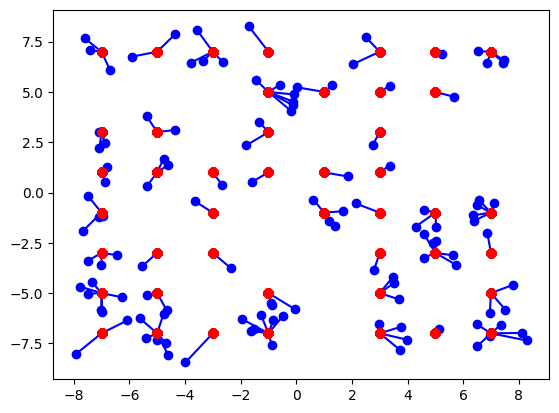
\includegraphics[width=0.7\linewidth]{../Source/results/Received-constellation.png}
    \caption{Received constellation and hard decision mapping}
    \label{received}
\end{figure}

Now, that the constellation is obtained back, we need to send the complex values to the demapper, to transform the constellation points to the bit groups. In order to do this, we compare each received constellation point against each possible constellation point and choose the constellation point which is closest to the received point. Then, we return the bit-group that belongs to this point. In the Figure \ref{received} above, the blue points are the received QAM points, where as the the red points connected to them are the closest possible constellation points, and the bit groups corresponding to these red points are returned.

Finally, the bit groups need to be converted to a serial stream of bits, by means of parallel to serial conversion. Figure \ref{output} show The received data for 4 cases of SRN equals 0, 10, 20 and 30 db respectively.

\begin{figure}[htbp]
    \centering
    \begin{subfigure}[t]{.49\linewidth}
        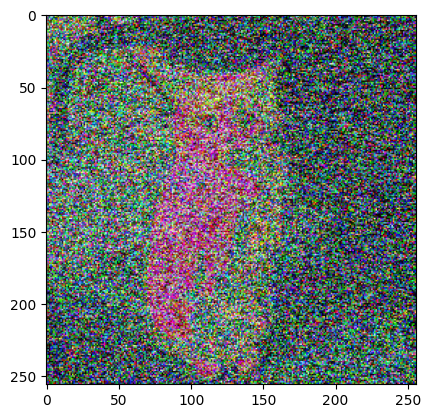
\includegraphics[width=\linewidth]{../Source/results/output_0db.png}
        \caption{SNR = 0db}
        \label{0db}
    \end{subfigure}
    \hfil
    \begin{subfigure}[t]{0.49\linewidth}
        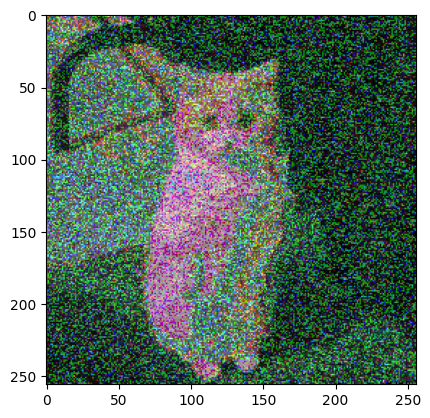
\includegraphics[width=\linewidth]{../Source/results/output_10db.png}
        \caption{SNR = 10db}
        \label{10db}
    \end{subfigure}
    \hfil
    \begin{subfigure}[t]{0.49\linewidth}
        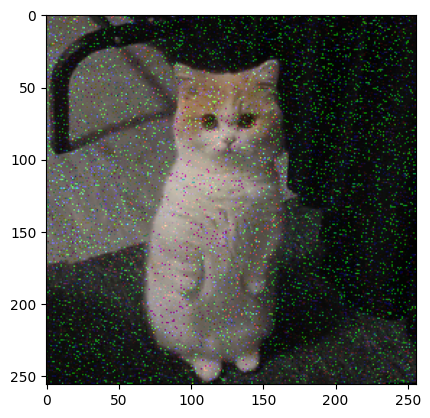
\includegraphics[width=\linewidth]{../Source/results/output_20db.png}
        \caption{SNR = 20db}
        \label{20db}
    \end{subfigure}
    \hfil
    \begin{subfigure}[t]{0.49\linewidth}
        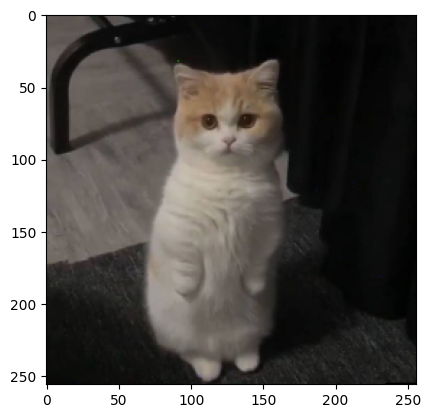
\includegraphics[width=\linewidth]{../Source/results/output_30db.png}
        \caption{SNR = 30db}
        \label{30db}
    \end{subfigure}
    \caption{The received using 64 QAM module}
    \label{output}
\end{figure}

\begin{figure}[htbp]
    \centering
    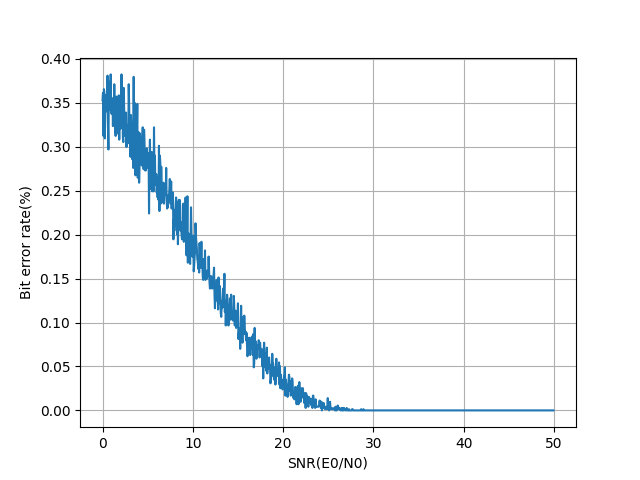
\includegraphics[width=\linewidth]{../Source/results/ber.png}
    \caption{Plot of BER for SNRdb values from 0 to 50}
    \label{ber}
\end{figure}
\newpage
\section*{CHAPTER 5: CONCLUSION}
\addcontentsline{toc}{section}{\numberline{}CHAPTER 5: CONCLUSION}
\setcounter{section}{2}
\setcounter{subsection}{0}
\setcounter{figure}{0}
\setcounter{table}{0}

An OFDM system is successfully simulated using Python in this project. All major components of an OFDM system are covered. This has demonstrated the basic concept and feasibility of OFDM, which was thoroughly described and explained in Chapter 3 of this report. Some of the challenges in developing this OFDM simulation program were carefully matching steps in modulator and demodulator, keeping track of data format and data size throughout all the processes of the whole simulation, designing an appropriate frame detector for the receiver, and debugging the MATLAB codes.

Chapter 4 showed and explained some analyses of the performance and characteristics of this simulated OFDM system.
\newpage



\phantomsection\addcontentsline{toc}{section}{\numberline {}REFERENCES}
% \bibliographystyle{IEEEtran}
% \bibliography{References}
\begin{thebibliography}{00}
\bibitem{b1} Schulze, Henrik and Christian Luders. Theory and Applications of OFDM and CDMA John Wiley \& Sons, Ltd. 2005
\bibitem{b2} Theory of Frequency Division Multiplexing
\bibitem{b3} Acosta, Guillermo. “OFDM Simulation Using MATLAB” 2000
\bibitem{b4} A Brief History of OFDM.
\bibitem{b5} Lui, Hui and Li, Guoqing. OFDM-Based Broadband Wireless Networks Design and Optimization Wiley-Interscience 2005
\bibitem{b6} Nguyen Van Duc. "Digital Communication Technique" 2004

\end{thebibliography}

\newpage
\section*{APPENDIX}
\phantomsection\addcontentsline{toc}{section}{\numberline{} APPENDIX}
\setcounter{section}{1}
\setcounter{subsection}{0}
\section*{Jupyter notebook for Simulation of the OFDM system using channel
coding, LMSE and 64 QAM modulation.}

\includepdf[
    pages=-,
    % pagecommand={\pagestyle{plain}},
    % addtotoc={1,section,1,APPENDIX,sec:apendix}
    ]
{../Source/build/OFDM.pdf}
\end{document}

